\subsection{RQ3: resource effects across offered load}\label{sec:load-results}
Figure~\ref{fig:load-sweep} reports all four offered rates and policies. At the upper rate, full retention consumes \LoadFullCPU{} Collector CPU-seconds, or \LoadFullCore{}\% of one core over the nominal 35-second window. Nominal 10\% tail uses \LoadTailCPU{}\,s, a paired increase of 59.1\%, while exported JSON falls to 10.9\% of full. Retain-all tail uses still more CPU despite identical retained span counts. Tail memory rises with offered load, consistent with the cost of retaining undecided trace state.

\begin{figure}[htbp]
\centering
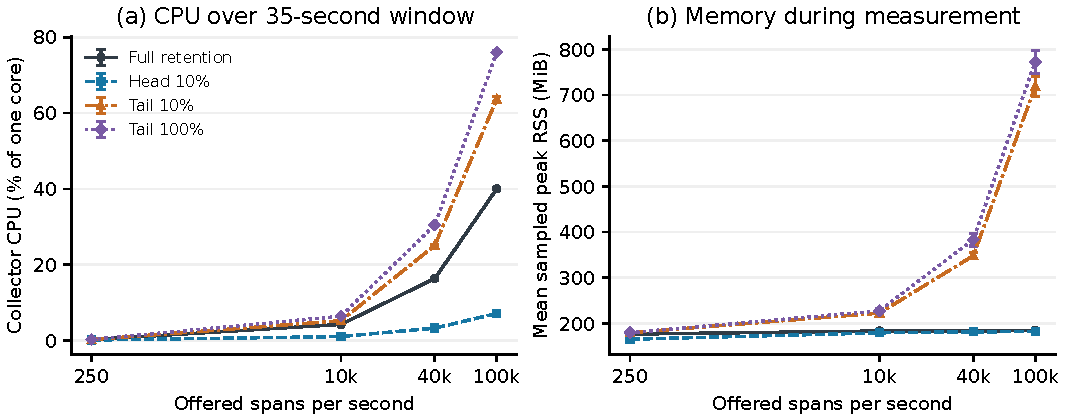
\includegraphics[width=\linewidth]{figures/load-sweep.pdf}
\caption{Collector load sweep with JSON file export, five runtime blocks per point. Error bars are pointwise 95\% Student-$t$ intervals. CPU refers to one core over the nominal 35-second window. Memory is mean per-cell sampled peak RSS. Capacity and batch settings are common across treatments. ``Head 10\%'' denotes the pre-ingress BLAKE2b gate; it is a different selection implementation from the matched controls in Table~\ref{tab:boundary}.}
\label{fig:load-sweep}
\end{figure}

At the upper rate, the pre-ingress gate saves \LoadHeadSaving{}\% of Collector CPU. Table~\ref{tab:load-high} reports all upper-rate treatments. The separate matched-placement experiment in RQ1, at 40,000 spans/s, demonstrates why a pre-ingress saving does not describe native probabilistic processing of full input; it is not a same-rate control for this 100,000-span/s point. For the tail path, avoided export work is insufficient to offset additional work at the upper JSON-only boundary. The fixed-input results in RQ2 establish that this sign is configuration-dependent.


\begin{table}[htbp]
\centering\small
\begin{tabular}{lrlrr}
\toprule
Policy & CPU (s) & CPU saving (\%, 95\% interval) & JSON (\%) & RSS (MiB) \\
\midrule
\tableinput{load-high-rows.tex}
\bottomrule
\end{tabular}
\caption{The separate load sweep at 100,000 offered spans/s, five paired blocks. CPU spans thirty seconds of offered load plus five seconds of drain. JSON is relative to full retention; RSS is the mean sampled per-cell peak. Negative savings mean greater cost. Head denotes the pre-ingress BLAKE2b gate.}
\label{tab:load-high}
\end{table}

All eighty cells reconcile complete selected traces, with no throttling, refusal, failed export, or early tail drop. These finite windows establish an observed operating point rather than a saturation limit.

\paragraph{SDK placement at a separate application boundary.}
The retained live application study supplies the SDK comparison. At fifty requests/s, SDK head sampling reduces combined gateway/worker process CPU by 15.4--18.0\% and Collector CPU by 31.3--36.5\% across its four application/traffic conditions (Table~\ref{tab:sdk-resources}). Those measurements include application execution and instrumentation, so their magnitudes differ from the pre-ingress gate's Collector-only savings. This separate experiment does not hold input or exporter configuration constant against the load sweep.

\begin{table}[htbp]
\centering\small
\begin{tabular}{lll}
\toprule
Application/traffic & Application CPU saving (\%) & Collector CPU saving (\%) \\
\midrule
\tableinput{sdk-resource-rows.tex}
\bottomrule
\end{tabular}
\caption{SDK head sampling at nominal 10\%, relative to full retention in the separate live study. Values are mean paired savings with pointwise 95\% intervals over five blocks. S denotes steady traffic and B bursty traffic. Application CPU sums the gateway and worker processes.}
\label{tab:sdk-resources}
\end{table}
